% Use only LaTeX2e, calling the article.cls class and 12-point type.

\documentclass[12pt]{article}

% Users of the {thebibliography} environment or BibTeX should use the
% scicite.sty package, downloadable from *Science* at
% www.sciencemag.org/about/authors/prep/TeX_help/ .
% This package should properly format in-text
% reference calls and reference-list numbers.

\usepackage{scicite}

% Use times if you have the font installed; otherwise, comment out the
% following line.

\usepackage{times}

% The preamble here sets up a lot of new/revised commands and
% environments.  It's annoying, but please do *not* try to strip these
% out into a separate .sty file (which could lead to the loss of some
% information when we convert the file to other formats).  Instead, keep
% them in the preamble of your main LaTeX source file.


% The following parameters seem to provide a reasonable page setup.

\usepackage{graphicx}

\topmargin 0.0cm
\oddsidemargin 0.2cm
\textwidth 16cm 
\textheight 21cm
\footskip 1.0cm


%The next command sets up an environment for the abstract to your paper.

\newenvironment{sciabstract}{%
\begin{quote} \bf}
{\end{quote}}


% If your reference list includes text notes as well as references,
% include the following line; otherwise, comment it out.

\renewcommand\refname{References and Notes}

% The following lines set up an environment for the last note in the
% reference list, which commonly includes acknowledgments of funding,
% help, etc.  It's intended for users of BibTeX or the {thebibliography}
% environment.  Users who are hand-coding their references at the end
% using a list environment such as {enumerate} can simply add another
% item at the end, and it will be numbered automatically.

\newcounter{lastnote}
\newenvironment{scilastnote}{%
\setcounter{lastnote}{\value{enumiv}}%
\addtocounter{lastnote}{+1}%
\begin{list}%
{\arabic{lastnote}.}
{\setlength{\leftmargin}{.22in}}
{\setlength{\labelsep}{.5em}}}
{\end{list}}


% Include your paper's title here

\title{Using \textit{MLFlow} to monitor an \textit{end-to-end} machine learning pipeline} 


% Place the author information here.  Please hand-code the contact
% information and notecalls; do *not* use \footnote commands.  Let the
% author contact information appear immediately below the author names
% as shown.  We would also prefer that you don't change the type-size
% settings shown here.

\author
{Vincent Dandenault,$^{1\ast}$ \\
\\
\normalsize{$^{1}$Department of Software Engineering, École de Polytechnique, Montréal}\\
\\
\normalsize{$^\ast$To whom correspondence should be addressed; E-mail: vincent.dandenault@polymtl.ca}
}

% Include the date command, but leave its argument blank.

\date{April 29th, 2020}



%%%%%%%%%%%%%%%%% END OF PREAMBLE %%%%%%%%%%%%%%%%



\begin{document} 

% Double-space the manuscript.

\baselineskip24pt

% Make the title.

\maketitle 



% Place your abstract within the special {sciabstract} environment.

\begin{sciabstract}
Machine Learning performs very well in labotory settings but doesn't seem transpose well into real world setting. Following this, the objective of this project was to use the tool \textit{MLFlow} to monitor and improve an existing machine learning model (Bayesian Netowrk) for the application Meditrinae. However, because of the immense number of parameters to track, it was impossible to use such a tool to imrpove the model's accuracy when tested with real world data. This paper is an overview of the process and a key insight into the problems we face in deploying machine learning models into production. 
  
\end{sciabstract}


\section*{Introduction}

Machinee Learning has been a \textit{hot topic} in the last decade as we've seeen its performance on specific tasks get better and better to a point of surpassing human capabilities, amoungs other, for image recognition. However, when trying to transpose these systems into real world applications and indstrial settings, regular and typical software engineering norms and principles seem to break down. 

In partnership with the \textit{Dental Faculty of the Univeristy of Toulouse}, my tream and I created the Meditrinae application that help dentists diagnos and treeat patients suffuring from temporo-mandibular disorders (DTM). The application works by collecting data entries of a patient (betweeen 100 and 150 answers) and then sent a Basian Network. Using imperial clinic knowledge, the bayesian network proposes a diagnostic based on the answer of the patient. 



\section*{Bayesian Network}

The basian network used in Medetrinae is a network with thousands of parameters that our the weights of the conditional probabilities. 

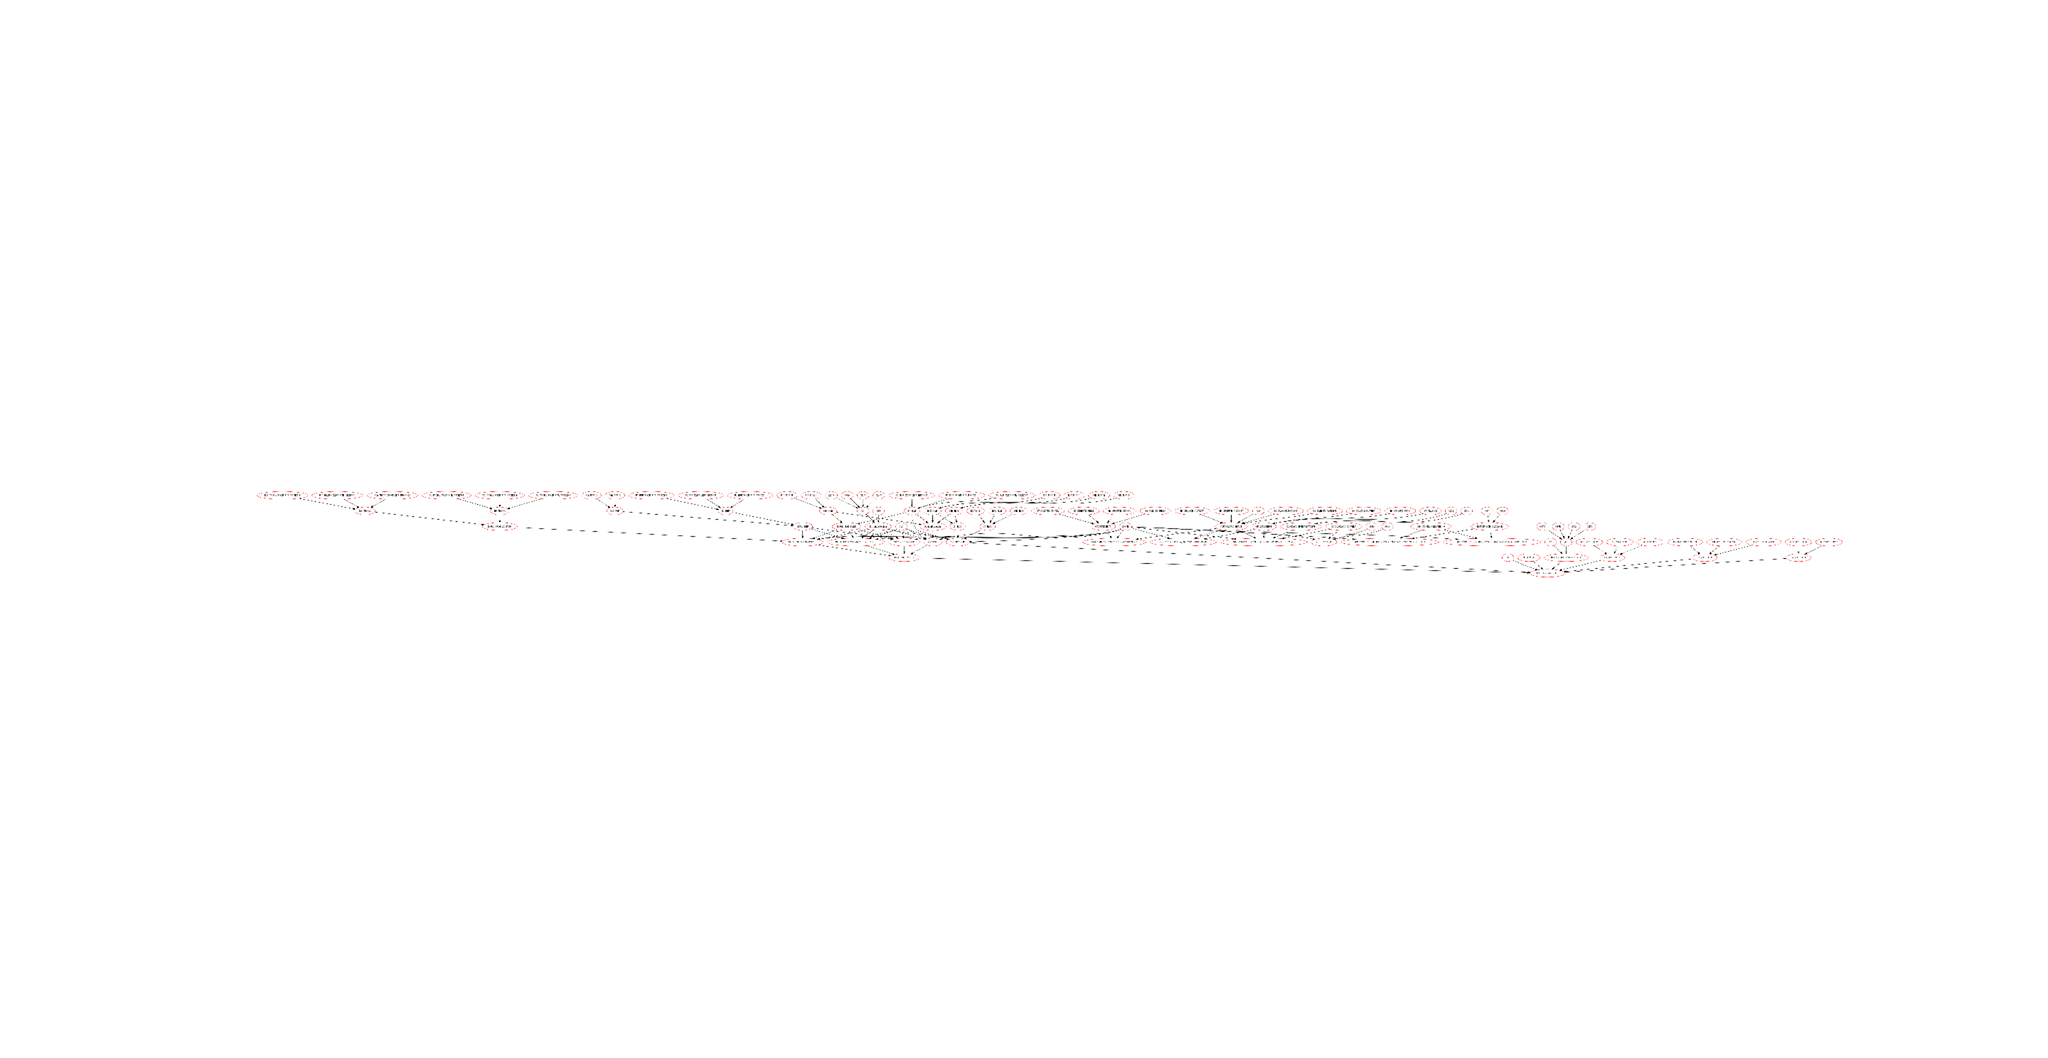
\includegraphics[scale=0.22]{model}

Theses parameters have underlying clinic significances and it has proven to be very difficult to group into hyperparameters. 

\section*{MLFlow}

MLFlow is a great tool to monitor the lifecycle of of a machine learning model  by versioning important parameters and the effects they have on the accuracy of the model. However, when trying to track thousands of parameters, the tool fails because it does not show a dependency between the chosen parameters and then accuracy of the model. Briefly, in Meditrinae's model, the lack of clairity from the parameters to show an increase of decrease in accuracy was very present. Moreover, it became impossible to version the training and the associated test sets. 

\section*{Conclusion}

In conclusion, the project did not succed as \textit{MLFlow} did not allow keeping track of the parameters used and it's corresponding accuracy changes. Furthermore, security concerns of the tool was a big problem and deployement on shared servers could not be achieve easily. 



\end{document}




















